\label{appendix:algorithm}

Presented here is a general approach to integrating nonlinear stochastic
partial differential equations. An integration scheme for the binary
XPFC equations of motion is presented as an application.

\section{Semi-Implicit Spectral Methods for Systems of First Order PDEs}  

To start, we consider the general case of time stepping  a system of non-linear
first-order PDE's. Specifically, we are going to look at a set of stochastic
non-linear PDE's,
%
\begin{equation}
	\f{\partial \vec{\psi}(x, t)}{\partial t} = 
       \mathcal{G}\l[ \vec{\psi}(x, t) \r] + \vec{\xi}(x, t),
\end{equation} 
%
Where,
\begin{description}[align=right, labelwidth=1cm]
    \item[$\vec{\psi}(x, t)$] {is a vector of our fields of interest (ex: (n, c))
        and we've used $\vec{\cdot}$ to denote a vector,
    }
    \item[$\mathcal{G}$] is some driving force for our fields and,
    \item[$\vec{\xi}(x, t)$] { is the stochastic driving force with 
        variances given by a generalized Einstein relationship.
    }
\end{description}

To develop a semi-implicit method we start by splitting the functional
$\mathcal{G}$ into linear and non-linear components, 
%
\begin{equation}
	\f{\partial \vec{\psi}(x, t)}{\partial t} = 
        \tn{\mathcal{L}}(x, x^\prime) \ast \vec{\psi}(x^\prime, t) 
	  + \mathcal{NL}\left[\vec{\psi}\right] + \vec{\xi}(x, t)
\end{equation} 
%
Where,
%
\begin{description}[align=right, labelwidth=1cm]
    \item[$\tn{\mathcal{L}}$]{denotes the linear contribution and $\tn{\cdot}$
        denotes a matrix,
    } 
    \item[$\ast$] {matrix multiplication and integration over
        the repeated variable and,}
    \item[$\mathcal{NL}$]{is the non-linear component of the the 
        functional $\mathcal{G}$.
    }
\end{description}
%
In a special set of PDE's the kernel $\tn{\mathcal{L}}$ is translationally
invariant. When this is the case, the convolution theorem can be used to write
the linear functional as an algebraic product in Fourier space. 
%
\begin{equation}
	\f{\partial \vec{\psi}(k, t)}{\partial t} = 
        \tn{\mathcal{L}}(k)\vec{\psi}(k, t) 
      + \mathcal{F}\left[\mathcal{NL}\left[\vec{\psi}\right]\right] 
      + \vec{\xi}(k, t)
\end{equation}
%
Where, $\mathcal{F}[\,\cdot\,]$ denotes a Fourier transform. We now consider
our fields on a discrete grid with $\Delta k$ spacing between Fourier modes and
$\Delta t$ spacing between times such that we might define, 
%
\begin{equation}
	\vec{\psi}_j^n \equiv \vec{\psi}(j\Delta k, n\Delta t). 
\end{equation}
%
To develop a generic approach to time stepping we consider evaluating our field
between grid points in time (eg. at $\vec{\psi}_j^{n + \gamma}$ where $\gamma
\in [0, 1]$). 
%
\begin{figure}[H]
	\label{schem}
	\begin{center}
	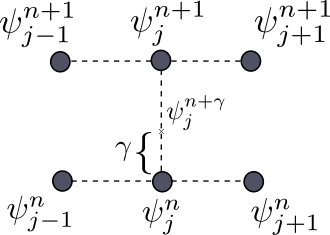
\includegraphics[scale=0.5]{algo_diagram.png}
	\end{center}
	\caption{Schematic of time step}
\end{figure}
%
To first order we can approximate this value as a linear interpolation of the
value at $n$ and the value at $n + 1$. 
%
\begin{equation}
	\vec{\psi}_j^{n + \gamma} = (1 - \gamma) \vec{\psi}_j^n 
        + \gamma \vec{\psi}_j^{n + 1}
\end{equation}
%
We can also approximate the time derivative $\partial_t \vec{\psi}$ as, 

\begin{equation}
	\f{\partial \vec{\psi}}{\partial t} = 
        \f{\vec{\psi}_j^{n+1} 
      - \vec{\psi}_j^n}{\Delta t} 
      + \f{1 - 2 \gamma}{2}\f{\partial^2 \vec{\psi}}{\partial t^2} \Delta t + ...
\end{equation}

Deriving different integration schemes is done by evaluating the equation of
motion for various values of $\gamma$. For example, to recover simple Euler
stepping we can evaluate the equation of motion with $\gamma = 0$. The
semi-implicit scheme relays on evaluating the non-linear component of the
equation of motion at $\gamma = 0$ while the rest of the equation is evaluated
at $\gamma = 1$. In this treatment we will evaluate the non-linear component at
$\gamma = 0$ but we will leave the rest of the equation unevaluated so that
$\gamma$ can be choosen freely at the end. Substituting these results into
equation of motion we find the following result, 
%
\begin{equation}
	  \f{\vec{\psi}_j^{n + 1} 
    - \vec{\psi}_j^{n}}{\Delta t}
    + \f{1 - 2\gamma}{2} \f{\partial^2 \vec{\psi}}{\partial t^2}\Delta t 
        = 
       \tn{\mathcal{L}} \left( (1 - \gamma) \vec{\psi}_j^n  
        + \gamma \vec{\psi}_j^{n+1} \right) 
     + \mathcal{F}\left[\mathcal{NL}\left[ \vec{\psi}_j^{n}\right]\right] 
     + \vec{\xi}_j^{n + \gamma}
\end{equation}
%
Separating $t=n+1$ terms on the left and $t=n$ terms on the right, 
%
\begin{equation}
	\left(\mathbb{1} - \Delta t  \gamma \tn{\mathcal{L}}\right) \vec{\psi}_j^{n + 1} 
		= \left(\mathbb{1} + \Delta t (1 - \gamma) \tn{\mathcal{L}}\right) \vec{\psi}_j^n 
		+ \Delta t \mathcal{F}\left[\mathcal{NL}\left[\vec{\psi}_j^n\right]\right] 
		+ \Delta t \vec{\xi}_j^{n + \gamma} 
		- \f{1 - 2\gamma}{2}\f{\partial^2 \vec{\psi}}{\partial t^2}\Delta t^2
\end{equation} 
%
Finally, we can isolate $\vec{\psi}_j^{n +1}$ by left multiplying by
$\left(\mathbb{1} - \gamma \Delta t \tn{\mathcal{L}}\right)^{-1}$, 
%
\begin{equation}
	\vec{\psi}_j^{n + 1} 
		=  \left(\mathbb{1} - \Delta t  \gamma \tn{\mathcal{L}}\right)^{-1} \left(
			\left(\mathbb{1} + \Delta t (1 - \gamma) \tn{\mathcal{L}}\right) \vec{\psi}_j^n 
			+ \Delta t \mathcal{F}\left[\mathcal{NL}\left[\vec{\psi}_j^n\right]\right] 
			+ \Delta t \vec{\xi}_j^{n + \gamma} 
			- \f{1 - 2\gamma}{2}\f{\partial^2 \vec{\psi}}{\partial t^2}\Delta t^2 
		\right)
\end{equation}
%
The final term on the right hand side emphasizes that if we choose $\gamma =
1/2$ we will have a algorithm that is accurate to second order in time (this is
a kind of Crank-Nicolson method). If we choose $\gamma = 1$ we recover a
semi-implicit method. 

%%%%%%%%%%%%%%%%%%%%%%%%%%%%%%%%%%%%%%%%%%%%%%%%%
\section{Applications to the Binary XPFC Model} %
%%%%%%%%%%%%%%%%%%%%%%%%%%%%%%%%%%%%%%%%%%%%%%%%%

The binary XPFC model is a good example of a system of first order PDE's like
those discussed in the previous discussion. The equations of motion in real
space are, 
%
\begin{align}
	\f{\partial c(x, t)}{\partial t} 
		&= M_c \nabla^2 \left( (\omega\epsilon - W_c\nabla^2) c 
			+ \omega (1 + n) \f{\partial \Delta F_{mix}(c)}{\partial c} 
			- \f{1}{2} n \left(\f{\partial C_{eff}}{\partial c} \ast n\right)
		\right) + \xi_c(x, t) \\
	\f{\partial n(x,t)}{\partial t} &= M_n \nabla^2 \left(
		\left(1 - C_{eff} \ast \right) n	- \f{\eta}{2} n^2 + \f{\chi}{3}n^3 + \omega\Delta F_{mix}
	 \right)  + \xi_n(x, t)
\end{align}
%
Where,
\begin{description}
    \item[$\Delta F_{mix}$] is the ideal free energy of mixing 
        $c\log\left(\f{c}{c_0}\right) + (1-c)\log\left(\f{1-c}{1-c_0}\right)$
\end{description}
%
With reference to the formalism we've already established our task is now to
seperate out the linear and non-linear components of these equations of motion.
To do this, we expand the concentration and density around constant references
$c_\ast$ and $n_\ast$. Doing so leads to an expression of $\tn{\mathcal{L}}$, 
%
\begin{equation}
	\tn{\mathcal{L}} =
    \begin{bmatrix}
	- M_c k^2 \l( \omega\l(\epsilon - \f{1}{c_\ast^2 - c_\ast}\r) + W_c k^2\r) & 
    - M_c k^2 \omega \log\l(\f{(c_0-1)c_\ast}{c_0(c_\ast-1)}\r) \\
	- M_n k^2 \omega \log \l(\f{(c_0-1)c_\ast}{c_0(c_\ast-1)}\r) &
    - M_n k^2 \l( 1-C_{eff}\vert_{c_\ast}(k) \r)
	\end{bmatrix}
\end{equation}
%
Important to note in the structure of $\tn{\mathcal{L}}$ is that it is diagonal
in the limit of small $\omega$. In the approximation that it is diagonal,
previous algorithms for the binary XPFC model are recovered where, to linear
order, concentration and density may be independently integrated. Another
interesting case is that of $M_n = M_c$ where the matrix is symmetric and thus
has orthogonal eigenvectors. We proceed by considering this simplified case
where the concentration and density are weakly coupled at the linear order and
may be integrated seperately.

%%%%%%%%%%%%%%%%%%%%%%%%%%%%%%%%%%%%%%%%%%%%%%%%%%%%%%%
\subsection{Algorithm for the Concentration $c(x,t)$} %
%%%%%%%%%%%%%%%%%%%%%%%%%%%%%%%%%%%%%%%%%%%%%%%%%%%%%%%

The concentration equation of motion is, 
%
\begin{equation}
    \partial_t \tilde{c} = 
        - M_c k^2\left(\omega\epsilon\tilde{c} 
        + W_c k^2\tilde{c} + \mathcal{F}\lbrace NL(c) \rbrace\right) 
        + \tilde{\xi}.
\end{equation}
%
Where $NL(c)$ is the non-linear term and $\xi$ is the drive noise. 
%
\begin{equation}
    NL(c) = 
        \omega(1+n)\l(\ln\l(\frac{c}{c_0}\r) 
      - \ln\l(\f{1-c}{1-c_0}\r)\r) 
      - \frac{1}{2} n \l(C_{eff}^n\ast n\r)
\end{equation}
%
Now if we think about the solution to this equation at time $t^{n+\xi}$ time
between $t^n$ and $t^{n+1}$ we express the solution as an interpolation between
the solutions at the earlier and later times.

\begin{equation}
    \tilde{c}_k^{n + \xi} = (1-\xi)\tilde{c}_k^n + \xi\tilde{c}_k^{n+1}
\end{equation}

We also find that we can express the time derivative as finite difference plus
a correction term. 

\begin{equation}
\partial_t \tilde{c} = \frac{\tilde{c}_k^{n+1} - \tilde{c}_k^{n}}{\Delta t} + 
\frac{1 - 2\xi}{2} \frac{\partial^2 \tilde{c}}{\partial t^2}\Delta t + ...
\end{equation}

Using each of these ideas we can rewrite the equation of motion completely,
with the exception of the nonlinear term, which we evaluate a the time $t^n$ in
keeping with many of the semi-implicit methods published.

\begin{equation}
\frac{\tilde{c}_k^{n+1} - \tilde{c}_k^{n}}{\Delta t} + 
\frac{1 - 2\xi}{2} \frac{\partial^2 \tilde{c}}{\partial t^2}\Delta t = 
\Lambda(k)\left[(1-\xi)\tilde{c}_k^n + \xi\tilde{c}_k^{n+1}\right] - M_c k^2 \mathcal{F}\lbrace NL(c^n)\rbrace + \tilde{\xi}_k^n
\end{equation}
where, 

\begin{equation}
\Lambda(k) = -M_c k^2\left(\omega\epsilon + W_c k^2\right).
\end{equation}

Moving future times to the left and past times to the right we find, 
%
\begin{equation}
    \tilde{c}_k^{n+1} = 
        \hat{P}\tilde{c}_k^n 
      + \hat{Q}\mathcal{F}\lbrace NL(c^n)\rbrace_k
      + \hat{L}\tilde{\xi}_k^n + \f{2\xi - 1}{2}
            \f{\partial^2 \tilde{c}}{\partial t^2}\Delta t^2
\end{equation}
%
Where the operators $\hat{P}$, $\hat{Q}$ and $\hat{L}$ are,
%
\begin{align}
    \hat{P} &= 1 + \frac{\Delta t \Lambda(k)}{1 - \xi\Delta t \Lambda(k)}  \\
    \hat{Q} &= -\frac{M_c k^2 \Delta t}{1 - \Delta t \xi \Lambda(k)} \\
    \hat{L} &= \frac{\Delta t}{1 - \Delta t \xi \Lambda(k)} 
\end{align}
%
Different values of $\xi$ lead to different integration schemes. The $\xi = 0$
corresponds to euler time stepping in fourier space, while $\xi = 1$ yields the
often used semi-implicit fourier method. There is an import case in which we
choose $\xi = 1/2$ where the algorithm becomes accurate to second order in
time. This is the Crank-Nicholson fourier method. 

%%%%%%%%%%%%%%%%%%%%%%%%%%%%%%%%%%%%%%%%%%%%%%%%%%%%%%%
\subsection{Algorithm for the Total Density $n(x,t)$} %
%%%%%%%%%%%%%%%%%%%%%%%%%%%%%%%%%%%%%%%%%%%%%%%%%%%%%%%

We can develop an algorithm for the equation of motion fo the total density in
the same way that we did with concentration. The equation of motion for the
total density in fourier space looks like, 

\begin{equation}
    \partial_t \tilde{n}(k, t) = 
        - M_n k^2 \left(\tilde{n} 
        + \mathcal{F}\lbrace NL(n)\rbrace\right) 
        + \tilde{\xi}
\end{equation}
%
Where now the nonlinear term is, 
%
\begin{equation}
    NL(n) = -\eta \f{n^2}{2} + \chi \f{n^3}{3}  + \Delta f_{mix}(c) - C_{eff}^n \ast n  
\end{equation}
%
Note that the convolution term is nonlinear because of an implicit dependance
on the concentration. Now, in principle, you could compute that pair
correlation function every time step for a more accurate linear propagator, but
here we will not consider that. 

Here again, we find the same structure as previously:
%
\begin{equation}
    \til{n}_k^{n+1} = 
        \hat{P}\til{n}_k^n 
      + \hat{Q}\mathcal{F}\lbrace NL(n^n)\rbrace_k
      + \hat{L} \til{\xi}_k
\end{equation}

Here, the operators $\hat{P}$, $\hat{Q}$ and $\hat{L}$ are:

\begin{align}
    \hat{P} &= 1 - \frac{\Delta t M_n k^2}{1 + \xi\Delta t M_n k^2}  \\
    \hat{Q} &= -\frac{M_c k^2 \Delta t}{1 + \Delta t \xi M_n k^2} \\
    \hat{L} &= \frac{\Delta t}{1 + \Delta t \xi M_n k^2} 
\end{align}

